\documentclass[11pt, a4paper]{article}
\usepackage{pdfpages}
\usepackage{parallel}
\usepackage[T2A]{fontenc}
%\usepackage{ucs}
\usepackage[utf8]{inputenc}
\usepackage[english,russian]{babel}
\usepackage{hyperref}
\usepackage{rotating}
\usepackage[inner=2cm,top=1.8cm,outer=2cm,bottom=2.3cm,nohead]{geometry}
%\usepackage{listings}
\usepackage{graphicx}
\usepackage{wrapfig}
\usepackage{longtable}
\usepackage{indentfirst}
\usepackage{array}
\usepackage{tikzsymbols}
\usepackage{soul}
\usepackage[ruled,vlined]{algorithm2e}
\usepackage{qrcode}
\counterwithout{figure}{section} 

\usepackage{url}
\makeatletter
\g@addto@macro{\UrlBreaks}{\UrlOrds}
\makeatother

\newcolumntype{P}[1]{>{\raggedright\arraybackslash}p{#1}}
\frenchspacing
%\usepackage{fixltx2e} %text sub- and superscripts
\usepackage{icomma} % коскі ў матэматычным рэжыме
%\PreloadUnicodePage{4}

\newcommand{\longpage}{\enlargethispage{\baselineskip}}
\newcommand{\shortpage}{\enlargethispage{-\baselineskip}}

\def\switchlang#1{\expandafter\csname switchlang#1\endcsname}
\def\switchlangbe{
\let\saverefname=\refname%
\def\refname{Літаратура}%
\def\figurename{Іл.}%
}
\def\switchlangru{
\let\saverefname=\refname%
\let\savefigurename=\figurename%
\def\refname{Литература}%
\def\figurename{Рис.}%
}
\def\switchlangen{
\let\saverefname=\refname%
\def\refname{References}%
\def\figurename{Fig.}%
}

\hyphenation{admi-ni-stra-tive}
\hyphenation{ex-pe-ri-ence}
\hyphenation{fle-xi-bi-li-ty}
\hyphenation{Py-thon}
\hyphenation{ma-the-ma-ti-cal}
\hyphenation{re-ported}
\hyphenation{imp-le-menta-tions}
\hyphenation{pro-vides}
\hyphenation{en-gi-neering}
\hyphenation{com-pa-ti-bi-li-ty}
\hyphenation{im-pos-sible}
\hyphenation{desk-top}
\hyphenation{elec-tro-nic}
\hyphenation{com-pa-ny}
\hyphenation{de-ve-lop-ment}
\hyphenation{de-ve-loping}
\hyphenation{de-ve-lop}
\hyphenation{da-ta-ba-se}
\hyphenation{plat-forms}
\hyphenation{or-ga-ni-za-tion}
\hyphenation{pro-gramming}
\hyphenation{in-stru-ments}
\hyphenation{Li-nux}
\hyphenation{sour-ce}
\hyphenation{en-vi-ron-ment}
\hyphenation{Te-le-pathy}
\hyphenation{Li-nux-ov-ka}
\hyphenation{Open-BSD}
\hyphenation{Free-BSD}
\hyphenation{men-ti-on-ed}
\hyphenation{app-li-ca-tion}

\def\progref!#1!{\texttt{#1}}
\renewcommand{\arraystretch}{2} %Іначай формулы ў матрыцы зліпаюцца з лініямі
\usepackage{array}

\def\interview #1 (#2), #3, #4, #5\par{

\section[#1, #3, #4]{#1 -- #3, #4}
\def\qname{LVEE}
\def\aname{#1}
\def\q ##1\par{{\noindent \bf \qname: ##1 }\par}
\def\a{{\noindent \bf \aname: } \def\qname{L}\def\aname{#2}}
}

\def\interview* #1 (#2), #3, #4, #5\par{

\section*{#1\\{\small\rm #3, #4. #5}}
\ifx\ParallelWhichBox\undefined%
    \addcontentsline{toc}{section}{#1, #3, #4}%
\else%
\ifnum\ParallelWhichBox=0%
    \addcontentsline{toc}{section}{#1, #3, #4}%
\fi\fi%

\def\qname{LVEE}
\def\aname{#1}
\def\q ##1\par{{\noindent \bf \qname: ##1 }\par}
\def\a{{\noindent \bf \aname: } \def\qname{L}\def\aname{#2}}
}

\newcommand{\interviewfooter}[1]{
\vskip 1em
\noindent \textit{#1}
}

\AtEndDocument{\vfill\centering \qrcode{https://github.com/fiowro/mouses/blob/main/\jobname.pdf}}

\switchlang{ru}
\begin{document}

\title{1981 "--- Xerox Alto Optical Mouse}
\date{}
\maketitle
\selectlanguage{russian}

В марте 1973 года корпорация Xerox анонсировала компьютер Xerox Alto, считающийся первой рабочей станцией (или персональным компьютером), а также первым компьютером, оснащенным графическим интерфейсом пользователя \cite{wiki}. В комплекте с этой рабочей станцией поставлялась и первая в истории компьютеров серийная мышь, Xerox Alto Mouse (рис. \ref{fig:XeroxAltoPic}). Первоначальный вариант мыши на основе двух колес был через несколько лет модернизирован, и вместо колес стал использоваться шар. Но все равно эти мыши были не слишком надежными: судя по цитатам, приведенным в \cite{mouses}, они собирали грязь, быстро засорялись и переставали управлять курсором. Когда это случалось, пользователь Alto должен был отключить мышь, положить ее в коробку «Мертвые мыши» и взять прошедшую чистку мышь из коробки «Чистые мыши». При этом цена мыши составляла более 400 долларов.

Работа над оптической мышью была начата в районе 1980 года для решения двух задач: улучшить надежность (за счёт отсутствия других подвижных частей, кроме кнопок) и существенно понизить цену (за счёт интегрированного решения в виде единственной микросхемы). Результатом этих усилий стало последнее поколение мышей Alto "--- Xerox Alto optical mouse, представленное в 1981 году \cite{vlsi81}. Мышь оказалась очень удачной по сравнению со своими механическими предшественниками, поэтому ее конструкцию сразу же адаптировали для компьютеров Xerox Star, а позднее и для некоторых копировальных аппаратов компании \cite{mouses}.

\begin{figure}[h]
    \centering
    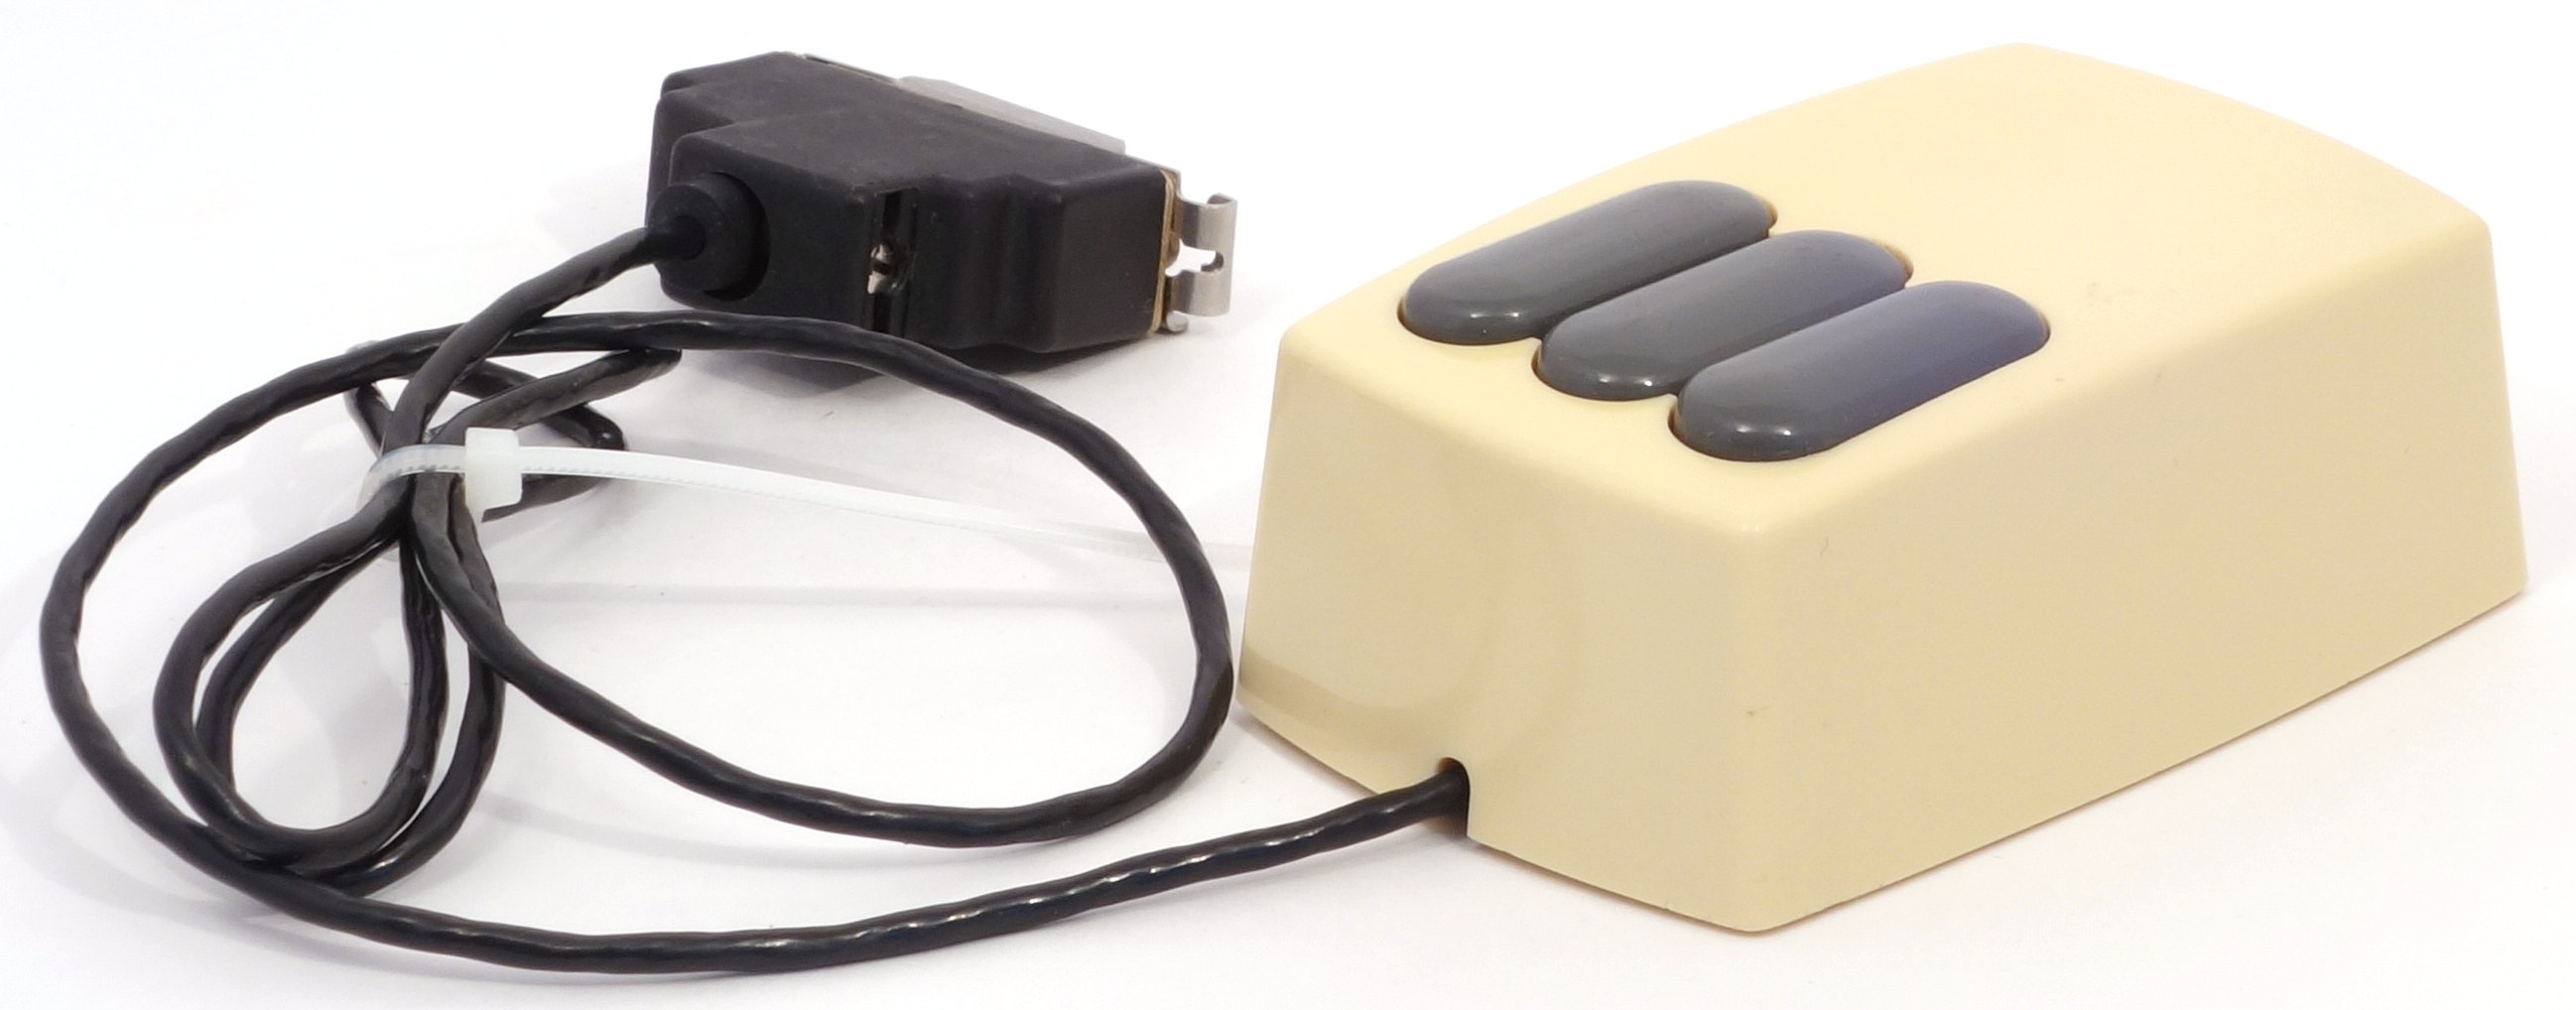
\includegraphics[scale=0.7]{1981_xerox_alto_mouse/pic_30.jpg}
    \caption{Xerox Alto Optical Mouse}
    \label{fig:XeroxAltoPic}
\end{figure}

Оптическая мышь Xerox Alto выполнена в том же корпусе, что и ее механическая версия \cite{vlsi82}, и имеет ту же цветовую схему. Корпус из кремового (исходно) пластика, в данной ревизии мыши глянцевого, представляет собой почти правильный паралеллепипед: слегка расширяется книзу и имеет выпуклые грани, чтобы уменьшить ассоциации с <<коробкой>>. В отличие от металлической нижней части механической мыши Alto, y оптического варианта низ выполнен из черного пластика, под цвет кабеля и разъема. На верхней стороне корпуса находятся три вытянутые закругленные кнопки, которые смыкаются краями, образуя визуально один цельный блок (рис. \ref{XeroxAltoTopAndBottom}).  В документации программного обеспечения Xerox кнопки мыши были обозначены как <<красная>>, <<желтая>> и <<синяя>>. Однако во всех случаях (кроме самой ранней модификации мыши с колёсами и поперечно расположенными кнопками \cite{vlsi81}), все три  изготавливались из черного (позднее, темно-серого) пластика. Вероятно, путаница, возникавшая у пользователей из-за такого неудачного цветокодирования, и поспособствоала мифу о преимуществе однокнопочных и двухкнопочных мышей перед мышами с тремя кнопками.

\begin{figure}[h]
    \centering
    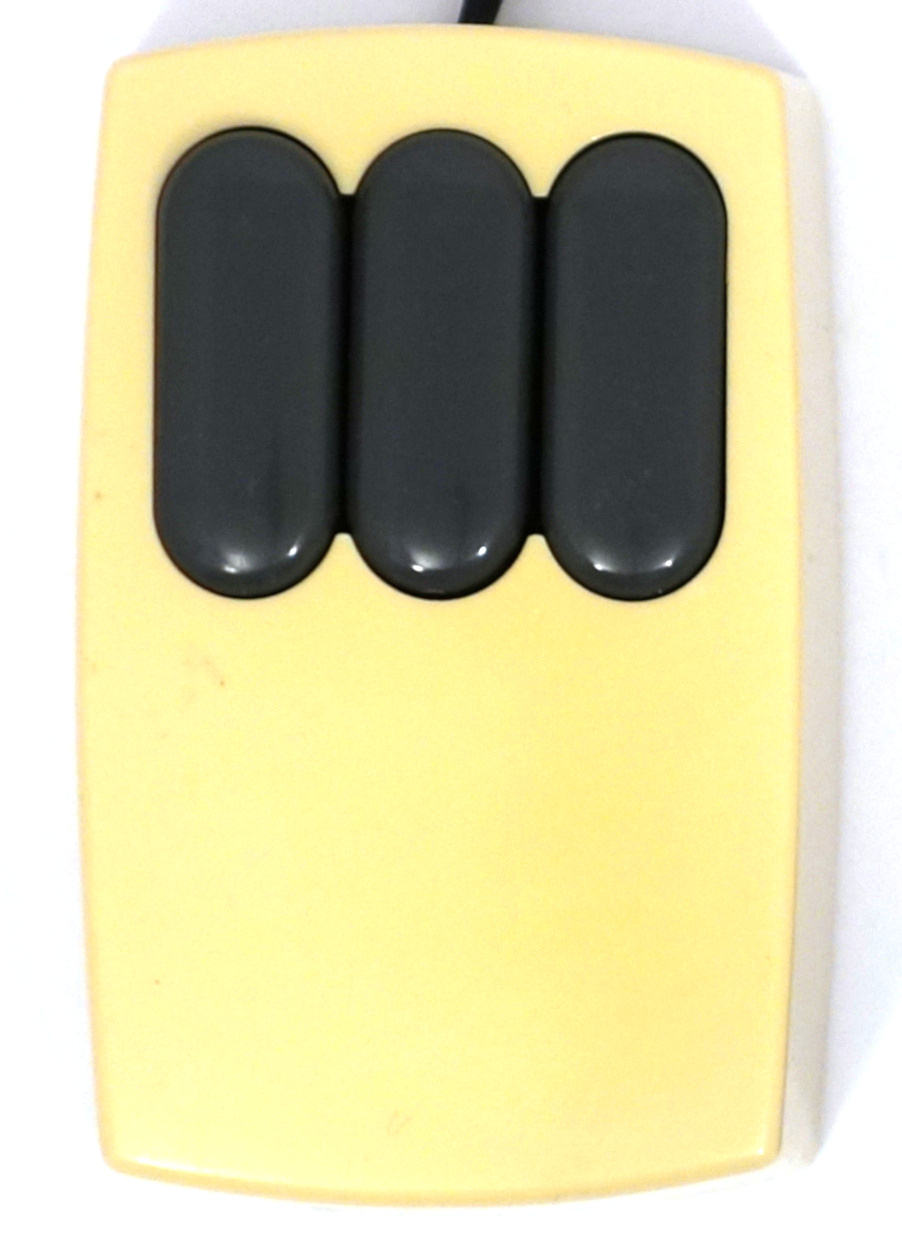
\includegraphics[scale=0.5]{1981_xerox_alto_mouse/top_30.jpg}
    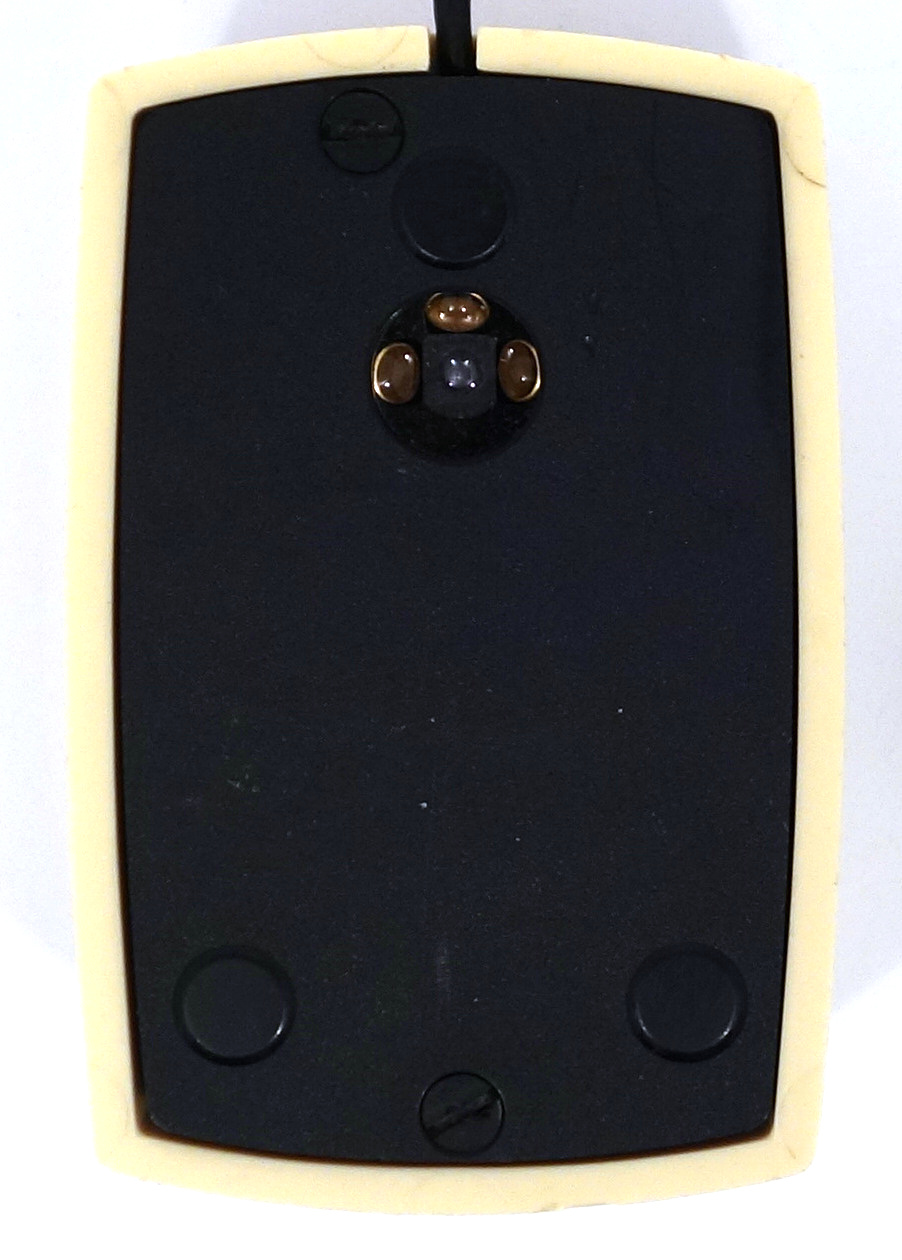
\includegraphics[scale=0.5]{1981_xerox_alto_mouse/bottom_30.jpg}
    \caption{Xerox Alto Optical Mouse, вид сверху и снизу}
    \label{XeroxAltoTopAndBottom}
\end{figure}

За регистрацию смещения цветовых неоднородностей при движении мыши отвечает сканирующая матрица размером $4 \times 4$ элемента, поэтому мыши требовался либо коврик со специально разработанным рисунком, либо поверхность с похожим чередованием мелких светлых и темных пятен, например, джинсовая ткань. Коврик для оптической мыши Xerox Alto был бумажным и продавался в пачках по 25 листов \cite{pad}. Узор представлял собой массив светлых шестиугольников на темном поле и был легко воспроизводим ксерокопированием. Реконструированный коврик можно увидеть на рис. \ref{fig:XeroxAltoPad}.

\begin{figure}[h]
    \centering
    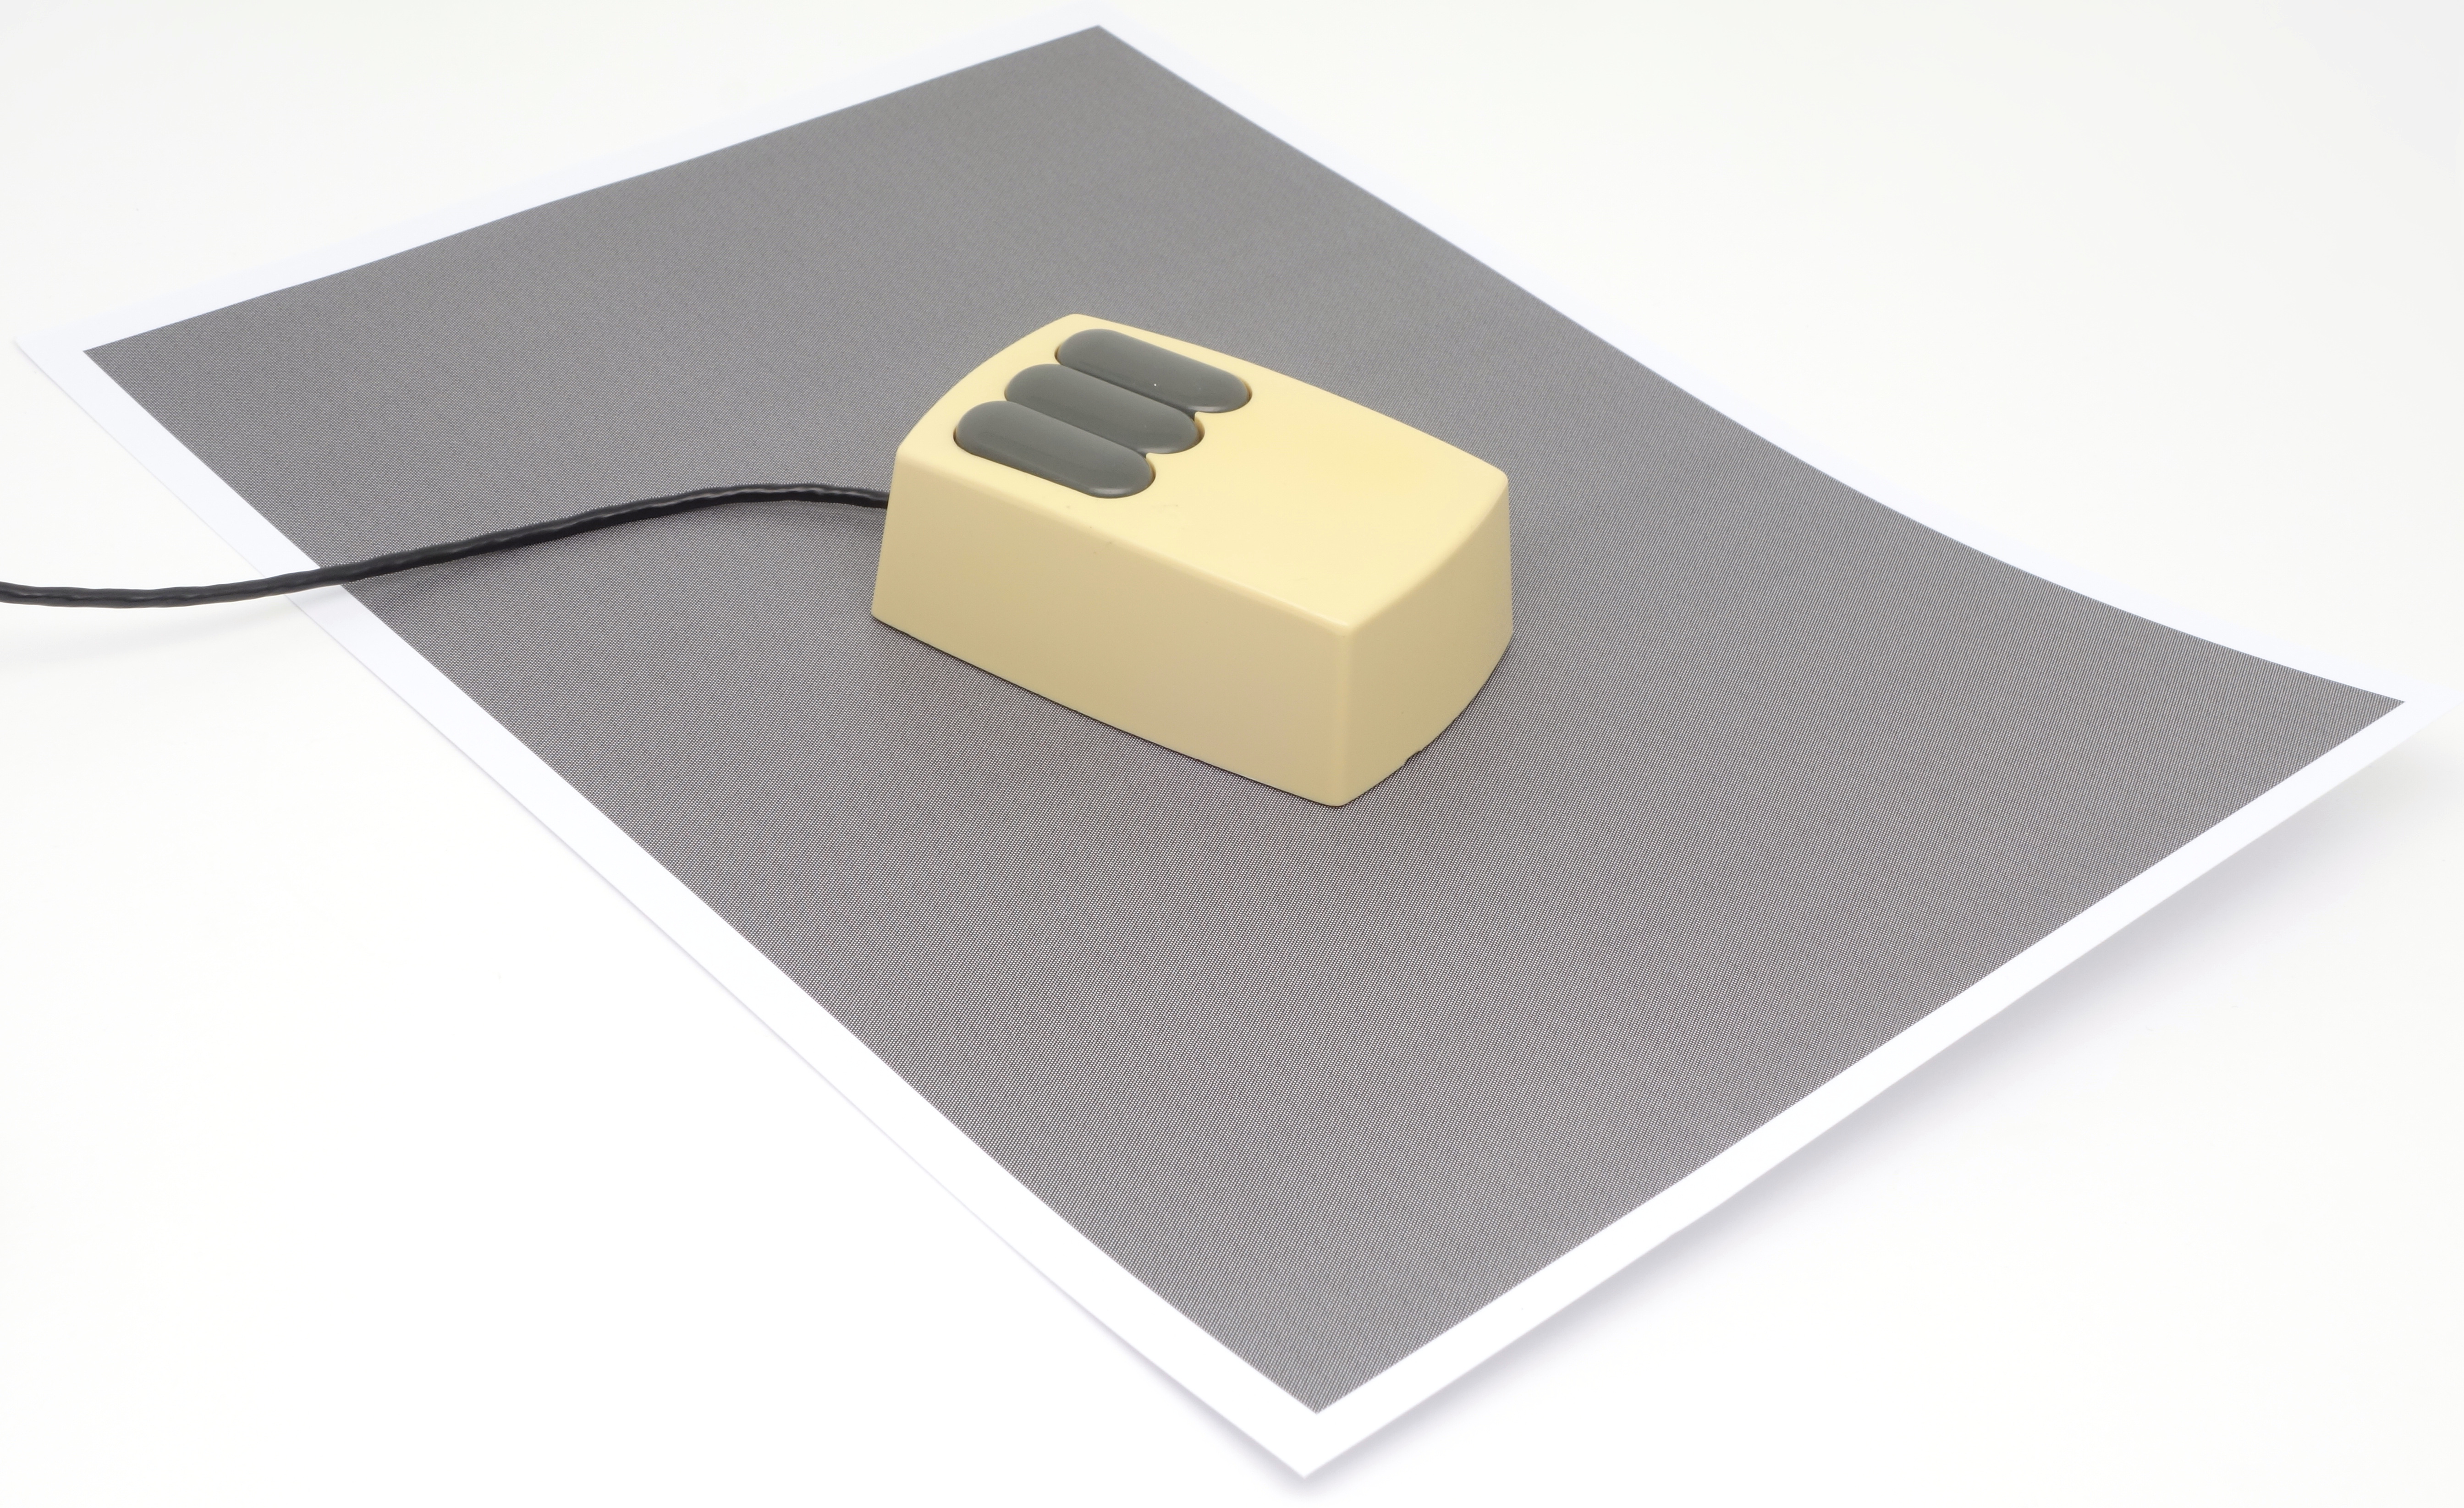
\includegraphics[scale=0.3]{1981_xerox_alto_mouse/pad_30.jpg}
    \caption{Xerox Alto Optical Mouse на реконструкции комплектного коврика}
    \label{fig:XeroxAltoPad}
\end{figure}

По размеру мышь могла бы быть меньше и ниже, если бы не использовала стандартный корпус мышей Alto. А так она получила типичные габариты для механических мышей  первой половины 80-х годов.

\begin{figure}[h]
    \centering
    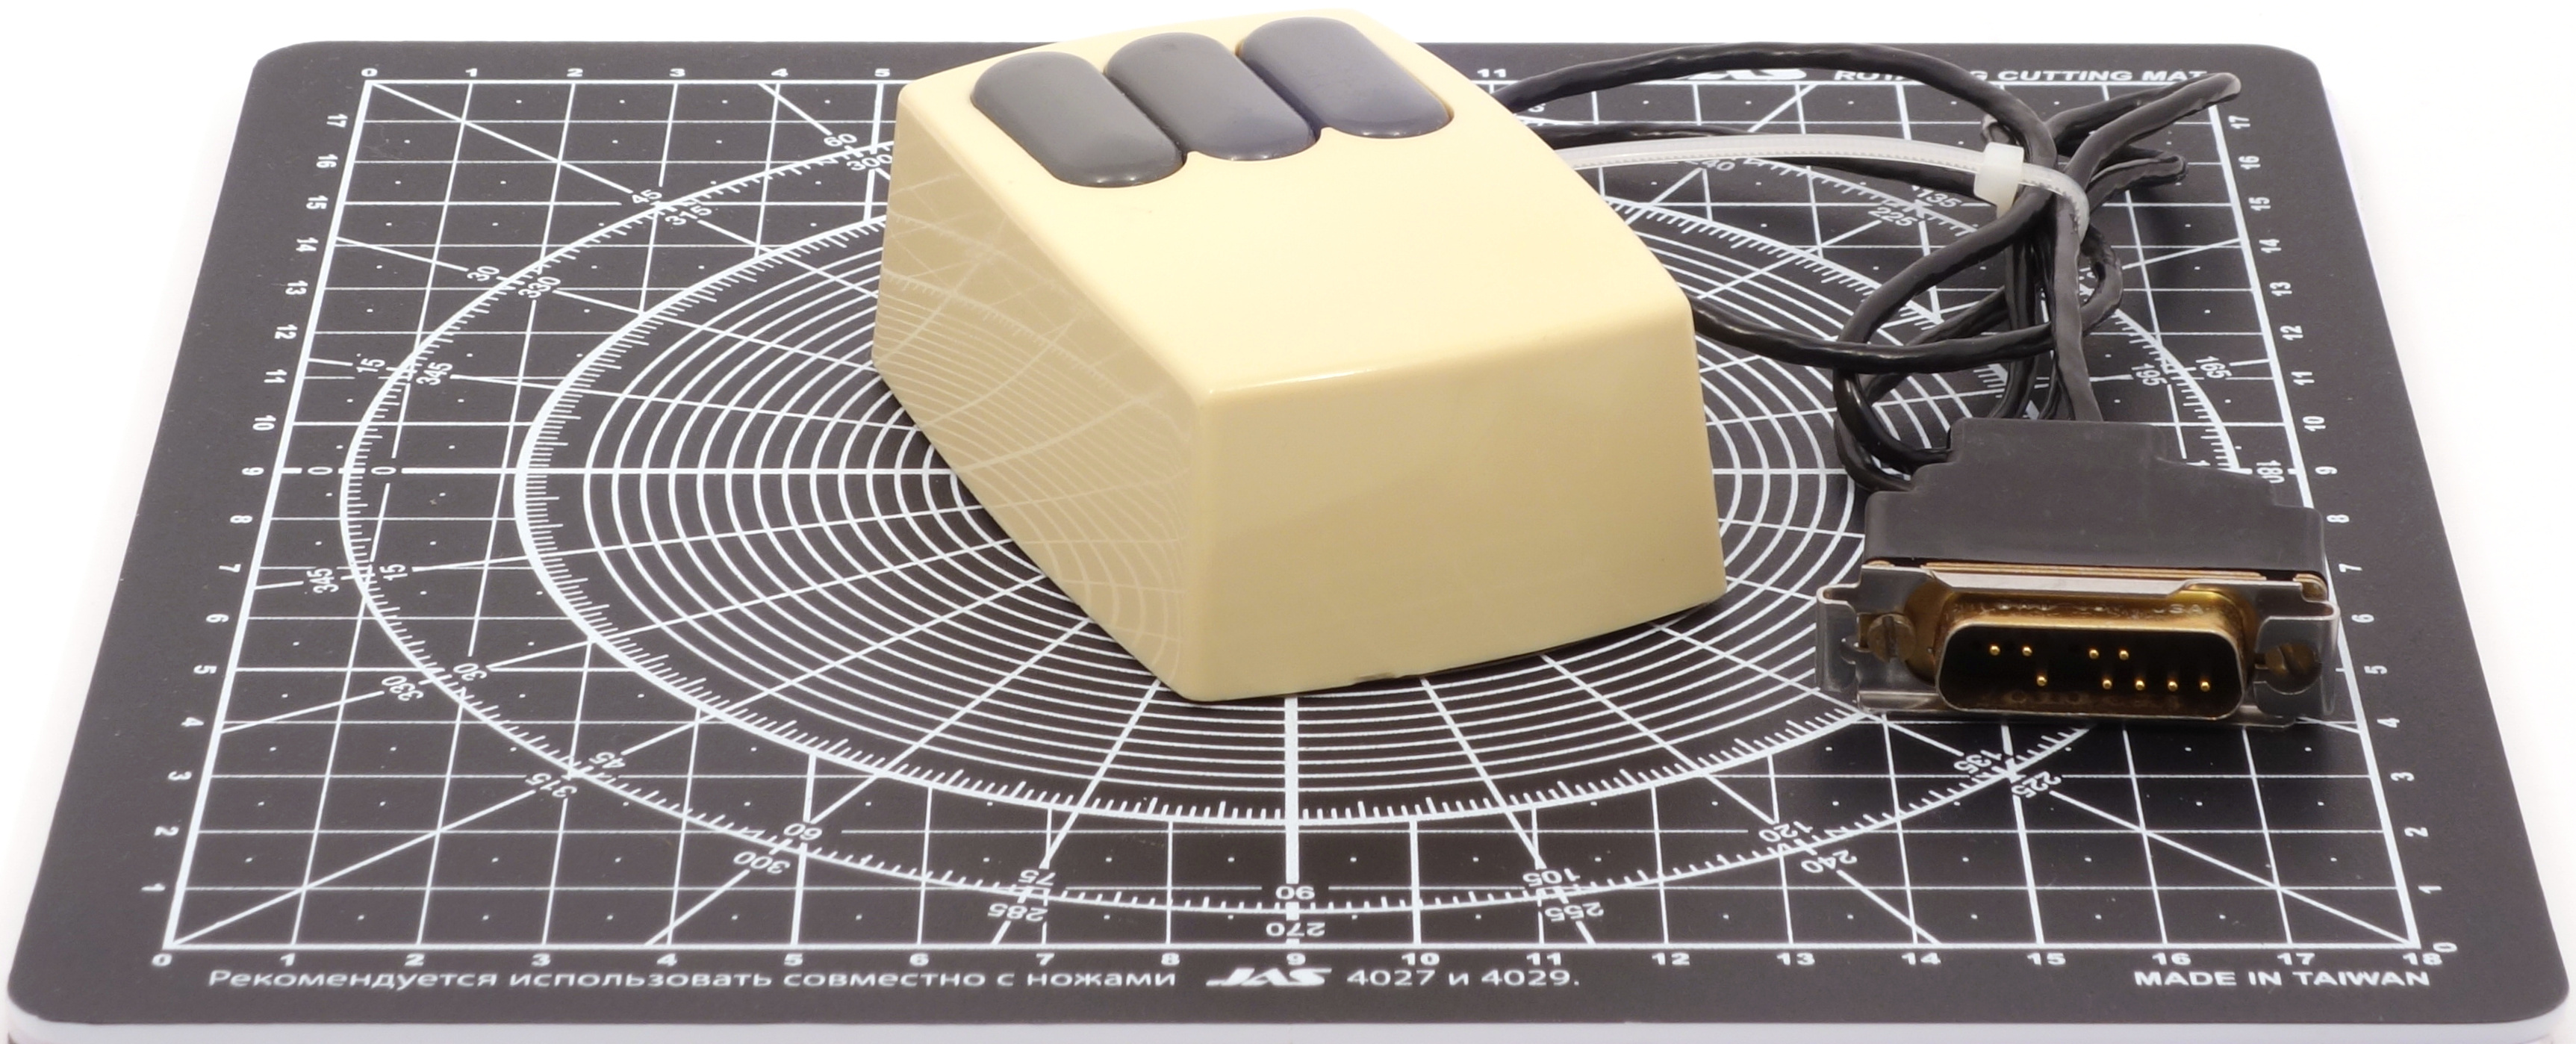
\includegraphics[scale=0.4]{1981_xerox_alto_mouse/size_15.jpg}
    \caption{Xerox Alto Optical Mouse на размерном коврике с шагом сетки 1~см}
    \label{fig:XeroxAltoSize}
\end{figure}

В плане эргономики и во внешнем виде Alto Mouse прослеживается минимализм. Пользовательский опыт несомненно страдает от суровой <<прямоугольности>> корпуса: её отчасти компенсируют выпуклые продолговатые кнопки, расположенные в зоне досягаемости пальцев, однако корпус не может обеспечить существенной поддержки ладони (рис. \ref{fig:XeroxAltoHand}).

\begin{figure}[h]
    \centering
    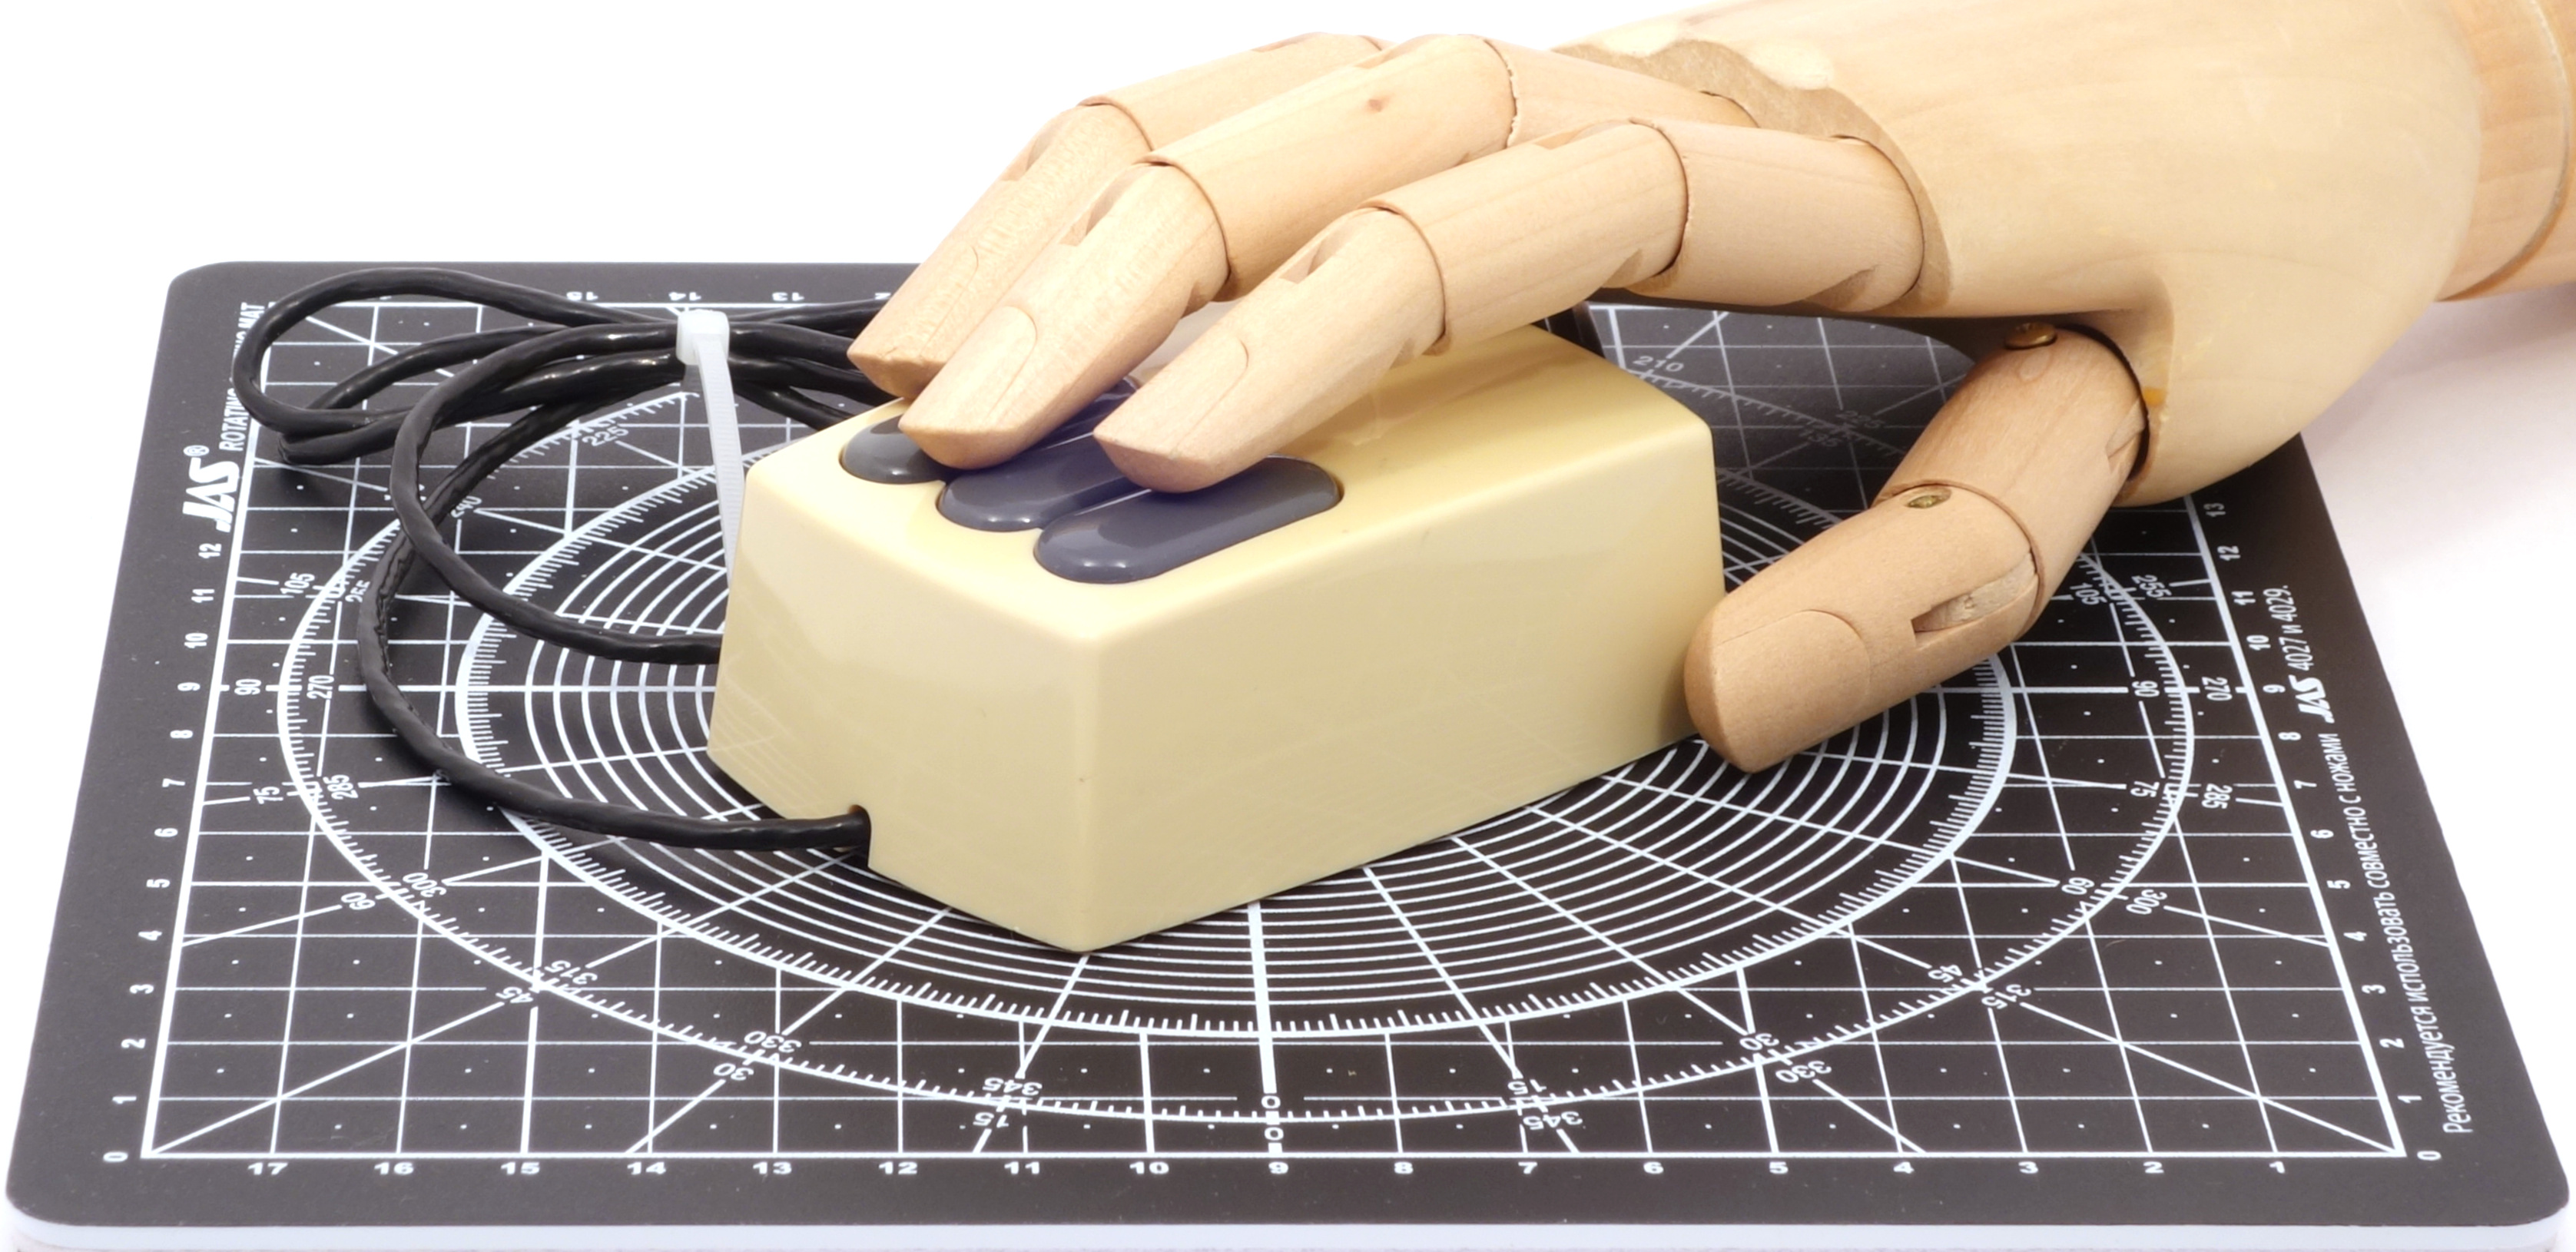
\includegraphics[scale=0.45]{1981_xerox_alto_mouse/hand_30.jpg}
    \caption{Xerox Alto Optical Mouse с моделью руки человека}
    \label{fig:XeroxAltoHand}
\end{figure}

Мышь имеет типичный для Xerox Alto разъем (в данном варианте "--- DA-15) и тот же квадратурный интерфейс, что и другие мыши Xerox. В разобранном виде манипулятор показан на рис. \ref{fig:XeroxAltoInside}, где можно увидеть пластиковый блок, зарывающий сканирующую матрицу от возможной засветки (в более поздних вариантах мышей для Xerox Star от него отказались), а также микросхему, отвечающую за обработку сигналов и выдачу квадратуры. Печатная плата поднята над основанием корпуса на вертикальных стойках, а под ней расположены под углом светодиоды для подсвечивания коврика мыши.

\begin{figure}[h]
    \centering
    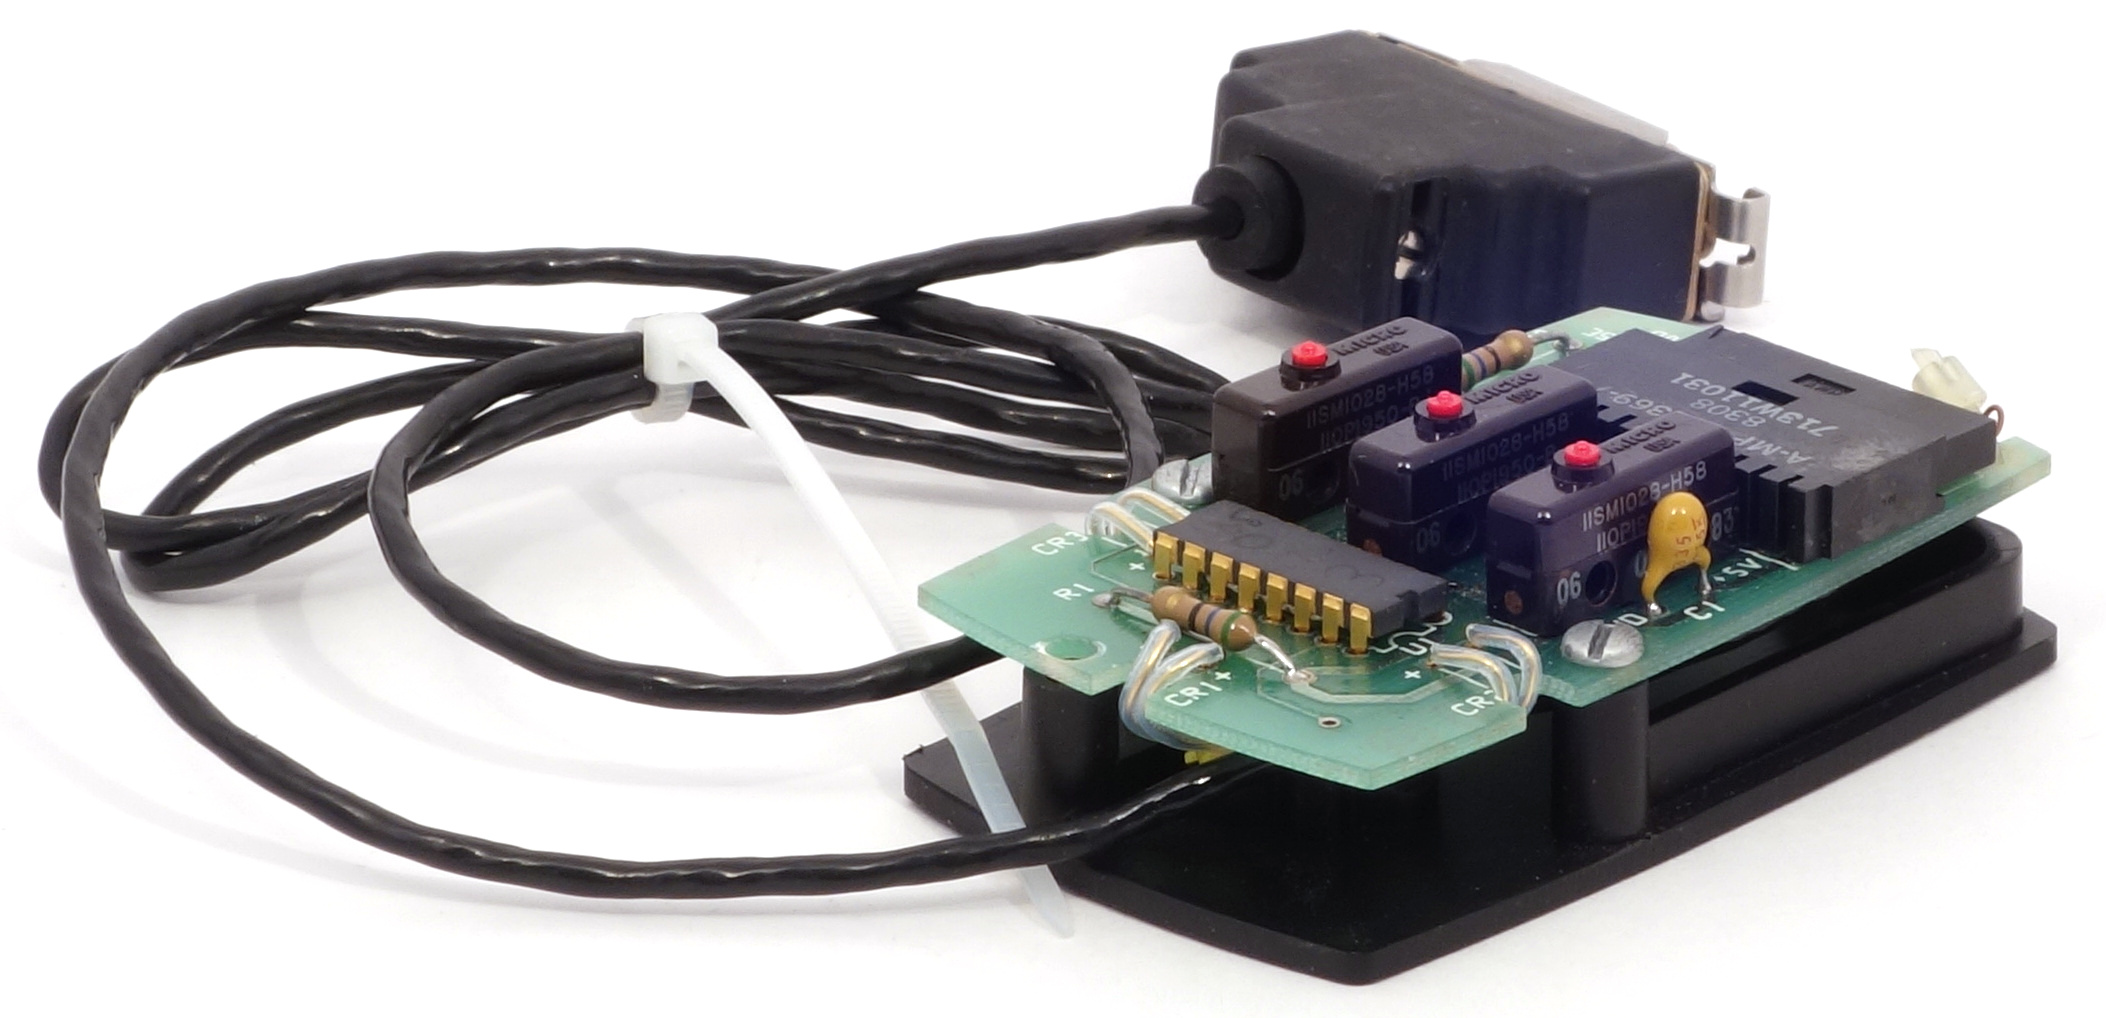
\includegraphics[scale=0.9]{1981_xerox_alto_mouse/inside_60.jpg}
    \caption{Xerox Alto Optical Mouse в разобранном виде}
    \label{fig:XeroxAltoInside}
\end{figure}

\begin{thebibliography}{9}
\bibitem {wiki} Xerox Alto: Wikipedia \url{https://en.wikipedia.org/wiki/Xerox_Alto}
\bibitem {vlsi81} R.\,F. Lyon. The Optical Mouse, and an Architectural Methodology for
Smart Digital Sensors // VLSI DESIGN, August 1981. - p. 20--30. \url{https://www.dicklyon.com/tech/OMouse/OpticalMouse-Lyon.pdf}
\bibitem {vlsi82} R.\,F. Lyon, M.\,P. Haeberli. Designing and Testing The Optical Mouse // VLSI DESIGN, January/February, 1982. - p. 20--30. \url{https://www.dicklyon.com/tech/OMouse/DesigningTestingOMouse.pdf}
\bibitem{pad} R.\,F. Lyon The Optical Mouse: Early Biomimetic Embedded Vision / Advances in Embedded Computer Vision, Nov 2014, pp.3-22 \url{https://static.googleusercontent.com/media/research.google.com/ru//pubs/archive/43260.pdf}
\bibitem{mouses} Xerox Mice. oldmouse.com \url{https://web.archive.org/web/20210418000634/http://oldmouse.com/mouse/xerox/alto.shtml}
\end{thebibliography}
\end{document}
